\documentclass{article}
%\usepackage[french]{babel}
\usepackage[utf8]{inputenc}
\usepackage{graphicx}
\graphicspath{ {images/}}
 \usepackage{wrapfig}
\usepackage{amsthm}
\usepackage{amssymb}
\usepackage{amsfonts}

\title{TP 1}
\author{SABABADY Kamala et SELVARAJAH Dinusan}

\begin{document}
\maketitle

\section{Partie 1 : $ f(x)= x^2-x-1$}

	Tout d'abord nous avons commencé par définir la fonction f(x) sous forme d'une fonction python puis nous avons représenté la fonction
$ f(x)= x^2-x-1$ sur l'intervalle [-1,2] en utilisant le module matplotlib.pyplot.

	On a pu observé que f possède deux racines qui sont environ  1.6 et -0.6. 


    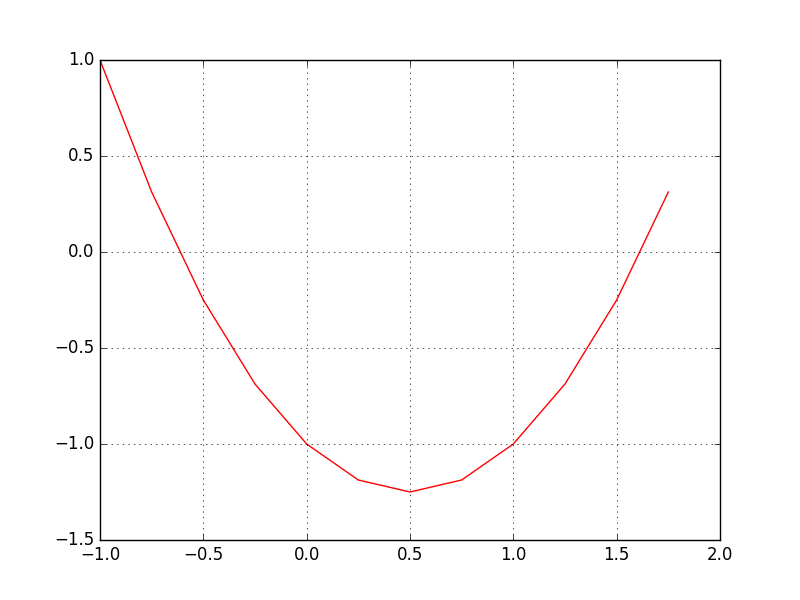
\includegraphics[width=10cm]{figure_1.png}



Nous avons pas eu de difficulté pour ces questions car dès le premier cours, on a compris comment on définit les fonctions sur python avec l'aide de l'enseignant puisque c'était les premiers pas sur le langage Python. Grâce a cela nous avons appris à définir les fonction sur python, afficher les graphiques, stoker les valeurs sur une listes.


\section{Partie 2 : $ g(x) = 1+1/x$ }
	
  Nous avons défini la fonction g comme pour la première partie. On a utilisé la commande np.arrange(x.debut,x.fin.pas) afin de remplacer la boucle while et c'est plus court. En utilisant la commande for i in range on  a pu vérifier les 25 premiers termes définie par la fonction g(x). Voici ci-dessous la vérification :

$$f(x) = 0 <=> x^2-x-1 = 0$$
$$         <=>  x^2-x = 1  $$
$$         <=>  x-1 = 1/x $$ 
$$         <=>  x = 1+1/x = g(x)$$	

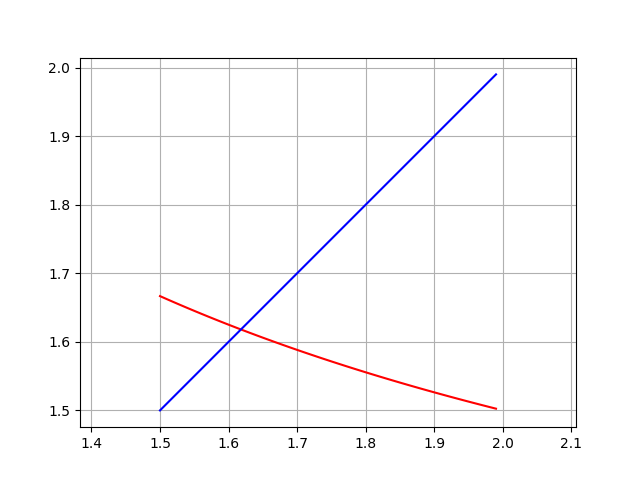
\includegraphics[width=10cm]{figure_1-2.png}
	$$ $$
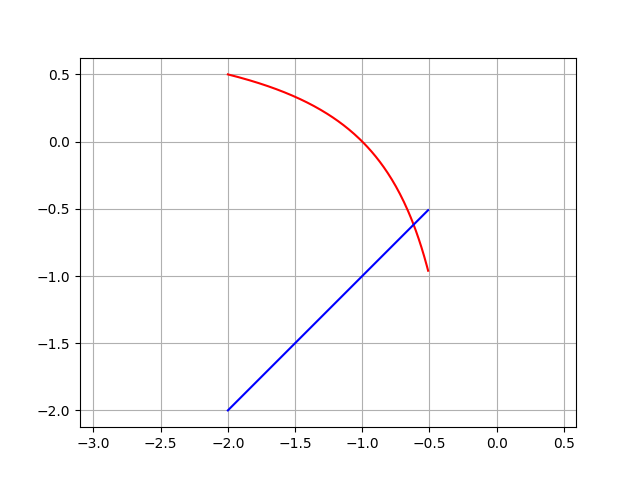
\includegraphics[width=10cm]{figure_131.png}

	Donc les points de g sont bien les zéros de f.
Nous avons crée une fonction pour calculer les 25 premiers termes de la suite. Au début, on a eu des problèmes pour l'exécution car souvent on a oublié ":", ou des "." et même un "print", problème de syntaxe. sinon on a réussi à faire afficher les 25 premiers termes de la suite $x(n+1)=g(xn) et x_{0}=1.0$. 

On observe que la suite converge vers le nombre d'or de la fonction f c'est à dire environ 1.62.

\section{Partie 3: Point fixe}
	Cette partie a été l'une des parties les plus difficiles car pour la fonction du point fixe, nous avons pris beaucoup plus de temps pour le faire puisque nous n'avons pas eu d'idée comment le programmer.
On a eu des problèmes de syntaxe, puis problème sur la condition d'arrêt du programme:$$\left|x_{n+1}-x_{n}\right| < \epsilon$$

 Après plusieurs test, nous avons réussi à compiler le programme. 
	on a fait le premier test avec $g(x) = 1 + 1/x, x_{0} = 1.0, \epsilon = 10^{12}$ puis avec $g(x) = 1 + 1/x, x_{0} = -0.6,  \epsilon = 10^{12}$.
 on remarque que la méthode de point fixe converge vers 1.62.
	Le problème de cette méthode c'est qu'elle converge que vers le nombre d'or (la racine positive de la fonction f) avec les deux test que nous avons tester. En fait, peut importe le nombre de départ 1.0 ou -0.6 cette méthode converge vers le même nombre qui est 1.61.

    \begin{wrapfigure}{l}{0.55\textwidth}
    \centering
    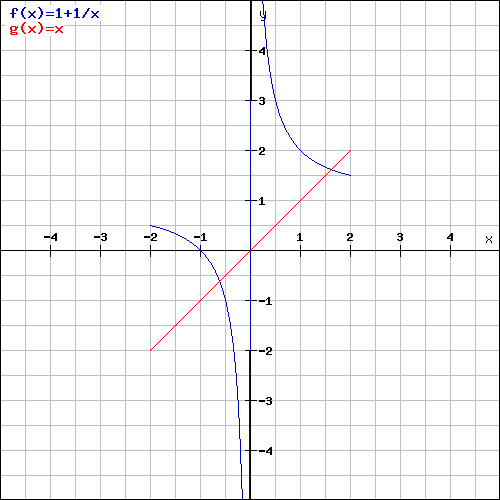
\includegraphics[width=0.55\textwidth]{graph.png}
\end{wrapfigure}
$$ $$


On voit dans le graphique que la pente sur la partie négative est supérieure à 1 $\left|g'(x)\right|> 1$ donc ce point fixe est répulsif.
Par contre la pente de la tangente sur la partie positive de l'intervalle est inférieure à 1 $\left|g'(x)\right|< 1$donc ce point fixe est attractif


    $$ $$
$$ $$
$$ $$
$$ $$
$$ $$
$$ $$
$$ $$




\section{Partie 4: Newton}

\begin{wrapfigure}{l}{0.25\textwidth}
    \centering
    
\includegraphics[width=0.25\textwidth]{image1.jpg}

\end{wrapfigure}
$$ $$

La méthode de Newton est une méthode de résolution de l'équation f (x) = 0, à la différence avec le théorème du point fixe qui permet de résoudre numériquement $f (x) = x$.
 C'est une méthode itérative qui construit une suite d'approximations. Le principe est le suivant :

 - On choisit x0 proche de la racine cherche. 

  - On calcule par recurrence les termes de la suite : 
$x_{n+1} = x_{n} - \frac{f(x_{n})}{f'(x_{n})}$.
 		
$$ $$
La suite  $x_{n}$  converge, si tout se passe bien, très rapidement vers la racine cherchée.

Tout d'abord on a défini la dérivé de la fonction f (voir tp1.py l.157) car on a besoin de la dérivée pour pouvoir définir la méthode de Newton. 
Les erreurs que nous avons faites sont qu'au début nous avions oublié de définir la fonction de la dérivée de f(x) puis il y avait des petits problèmes de syntaxe par exemple oubli des guillemets ou même oubli de parenthèse . 

Vérifions si les points fixes de g sont bien les zéros de f:
$$ x-\frac{f(x)}{f'(x)}=x$$ 
$$ <=> \frac{f(x)}{f'(x)}=0$$
$$<=> f(x)=0 $$  car $f'(x) \neq  0 $
Donc on a bien les zéros de f.
$$ $$

\section{Partie 5: Sécante}
La méthode de la sécante est une méthode itérative où chaque approximation est construite à partir des deux approximations précédentes. 
On doit donc partir de deux valeurs initiales distinctes, $x_{0}$ , $x_{1}$ (en général les bornes d’un encadrement de la racine cherchée), puis on calcule par récurrence les termes de la suite 

$$x_{n+1} = x_{n}-\frac{(x_{n}-x_{n-1})}{f(x_{n})-f'(x_{n-1})} f(x_{n})$$. 

L’avantage sur la méthode de Sécante est qu’on n’a pas besoin de la dérivée de f.
Au début, on a eu des problème pour comprendre la méthode puis à l'aide de nos camarades, on a réussi à comprendre et à compiler notre programme.

 
\section{Partie 6: Dichotomie}

Tout d'abord, pour cette partie nous n'avons pas eu de difficultés car la méthode de dichotomie est la méthode la plus simple à comprendre et à exécuter le programme. De plus nous avons fait des recherches sur internet pour nous aider. Nous avons terminer cette méthode en premier. 

Notre programme est une fonction récursive en effet, la fonction prend en arguments une fonction, deux valeurs initiales a et b, et un réel positif (epsilon). il y a deux conditions, tout d'abord le programme renvoie les valeurs a et b si b-a est inférieur ou égale à epsilon sinon on crée un réel c qui est la moité de la somme des valeurs initiales  et on test si f(a)*f(c) est inférieur ou égale à 0 si c'est le cas le programme réexécute dichotomie avec comme valeurs a et b remplacé par c sinon il réexecute dichotomie avec comme valeurs a remplacé par c et b. 

Nous avons fait deux tests avec les valeurs données dans le TP et nous avons trouvé les racines de f. 

\section{Partie 7: La vitesse de convergence }
\begin{center}
\begin{tabular}{l | c c c c c}
{} & $10^{-3}$ & $10^{-6}$ & $10^{-9}$ & $10^{-12}$ & $10^{-15}$ \\
\hline
\texttt{point\_fixe} & {9} & {16} & {23} & {30} & {38} \\
\texttt{newton} & {5} & {5} & {6} & {6} & {7} \\
\texttt{secante} & {6} & {7} & {8} & {8} & {FAULT} \\
\texttt{dichotomie} & {1} & {1} & {1} & {1} & {1} 
\end{tabular}
\end{center}

Pour la méthode de sécante avec $\epsilon = 10^{-15}$, le terminal affiche "float division by 0" , le problème vient du epsilon plus petit. Il n'y a pas assez de mémoire pour avoir une telle précision .
\end{document}

